\documentclass[a4paper,11pt]{jsarticle}


% 数式
\usepackage{amsmath,amsfonts}
\usepackage{bm}
% 画像
\usepackage[dvipdfmx]{graphicx}
\usepackage{here}

\usepackage[hang,small,bf]{caption}
\usepackage[subrefformat=parens]{subcaption}
\captionsetup{compatibility=false}


\begin{document}

\title{進捗報告}
\author{鷹見大地}
\date{\today}
\maketitle


\section{進捗}
\subsection{重み計算}
前回の計算の結果から、推定量から計算した重みが最適解になる可能性があることがわかったため、まずはパラメータを変化させその重みを計算しこれを検証した。

計算に用いたパラメータは以下の表\ref{table:1}および表\ref{table:2}の2通りである。

\begin{table}[H]
  \centering
  \caption{パターン1}
  \begin{tabular}{|c|c|c|c|c|c|}
  \hline
        & $\bar{k}$ & $\hat{S_1}$ & $\hat{S_2}$ & $\tilde{S_1}$ & $\tilde{S_2}$ \\ \hline
  $k_t$    & 1.0     & 0.1       & 0.1       & 0           & 0           \\ \hline
  $k_{m1}$ & 1.0     & 0〜1       & 0.2       &             &             \\ \hline
  $k_{m2}$ & 1.0     & 0.2       & 0.1       &             &             \\ \hline
  \end{tabular}
  \label{table:1}
\end{table}

\begin{table}[H]
  \centering
  \caption{パターン2}
  \begin{tabular}{|c|c|c|c|c|c|}
  \hline
        & $\bar{k}$ & $\hat{S_1}$ & $\hat{S_2}$ & $\tilde{S_1}$ & $\tilde{S_2}$ \\ \hline
  $k_t$    & 1.0     & 0〜1       & 0.1       & 0           & 0           \\ \hline
  $k_{m1}$ & 1.0     & 0.1       & 0.2       &             &             \\ \hline
  $k_{m2}$ & 1.0     & 0.2       & 0.1       &             &             \\ \hline
  \end{tabular}
  \label{table:2}
\end{table}

結果を図\ref{fig:3}および図\ref{fig:6}に示した。

\begin{figure}[H]
  \begin{tabular}{cc}
    \begin{minipage}[t]{0.45\hsize}
      \centering
      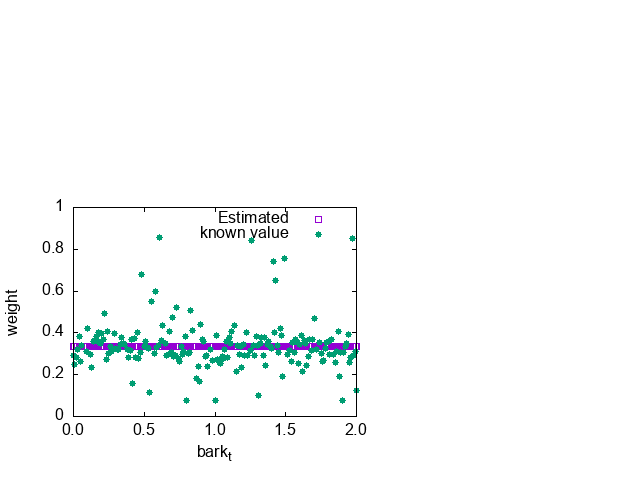
\includegraphics[keepaspectratio,scale=0.5]{weight1.eps}
      \subcaption{a1}
      \label{fig:1}
    \end{minipage} &
    \begin{minipage}[t]{0.45\hsize}
      \centering
      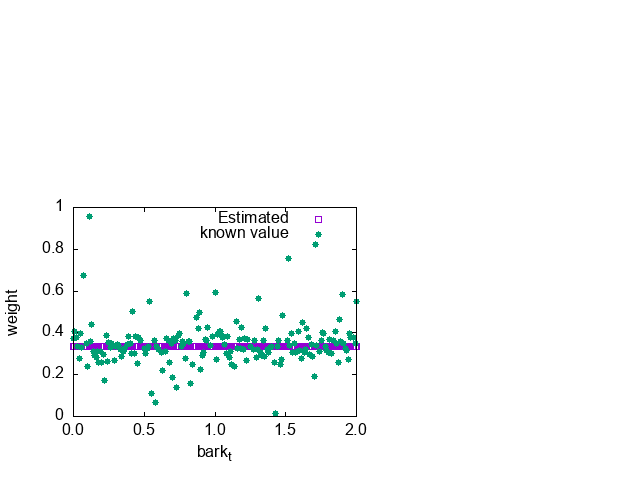
\includegraphics[keepaspectratio,scale=0.5]{weight2.eps}
      \subcaption{a2}
      \label{fig:2}
    \end{minipage} 
  \end{tabular}
  \caption{パターン1の結果}
  \label{fig:3}
\end{figure}

\begin{figure}[H]
  \begin{tabular}{cc}
    \begin{minipage}[t]{0.45\hsize}
      \centering
      \includegraphics[keepaspectratio,scale=0.5]{weight3.eps}
      \subcaption{a1}
      \label{fig:4}
    \end{minipage} &
    \begin{minipage}[t]{0.45\hsize}
      \centering
      \includegraphics[keepaspectratio,scale=0.5]{weight4.eps}
      \subcaption{a2}
      \label{fig:5}
    \end{minipage} 
  \end{tabular}
  \caption{パターン2の結果}
  \label{fig:6}
\end{figure}

この結果から、どの値においても計算結果は期待される重みを示すことがわかる。
よってこの時点では無次元化の操作をせず、この値をそのまま用いるのが良いのではないかと考えた。

続いて、$\tilde{St}$を効かせた場合を計算した。条件は以下の表に示した。

\begin{table}[H]
  \centering
  \caption{パターン1}
  \begin{tabular}{|c|c|c|c|c|c|}
  \hline
        & $\bar{k}$ & $\hat{S_1}$ & $\hat{S_2}$ & $\tilde{S_1}$ & $\tilde{S_2}$ \\ \hline
  $k_t$    & 1.0     & 0.1       & 0.1       & 0.01           & 0.01           \\ \hline
  $k_{m1}$ & 1.0     & 0〜1       & 0.2       &             &             \\ \hline
  $k_{m2}$ & 1.0     & 0.2       & 0.1       &             &             \\ \hline
  \end{tabular}
  \label{table:6}
\end{table}

\begin{table}[H]
  \centering
  \caption{パターン2}
  \begin{tabular}{|c|c|c|c|c|c|}
  \hline
        & $\bar{k}$ & $\hat{S_1}$ & $\hat{S_2}$ & $\tilde{S_1}$ & $\tilde{S_2}$ \\ \hline
  $k_t$    & 1.0     & 0〜1       & 0.1       & 0.01           & 0.01           \\ \hline
  $k_{m1}$ & 1.0     & 0.1       & 0.2       &             &             \\ \hline
  $k_{m2}$ & 1.0     & 0.2       & 0.1       &             &             \\ \hline
  \end{tabular}
  \label{table:7}
\end{table}

結果を以下の図に示した。

\begin{figure}[H]
  \begin{tabular}{cc}
    \begin{minipage}[t]{0.45\hsize}
      \centering
      \includegraphics[keepaspectratio,scale=0.5]{weight5.eps}
      \subcaption{a1}
    \end{minipage} &
    \begin{minipage}[t]{0.45\hsize}
      \centering
      \includegraphics[keepaspectratio,scale=0.5]{weight6.eps}
      \subcaption{a2}
    \end{minipage} 
  \end{tabular}
  \caption{パターン1の結果}
\end{figure}

\begin{figure}[H]
  \begin{tabular}{cc}
    \begin{minipage}[t]{0.45\hsize}
      \centering
      \includegraphics[keepaspectratio,scale=0.5]{weight7.eps}
      \subcaption{a1}
      % \label{fig:4}
    \end{minipage} &
    \begin{minipage}[t]{0.45\hsize}
      \centering
      \includegraphics[keepaspectratio,scale=0.5]{weight8.eps}
      \subcaption{a2}
      % \label{fig:5}
    \end{minipage} 
  \end{tabular}
  \caption{パターン2の結果}
  % \label{fig:6}
\end{figure}

\subsection{無次元化}
こちらは前回の結果で標準偏差が特殊な挙動を示したため、それの検証を行った。
まず、今までは$a_1$と$a_2$を同時に動かすパターンしか検証していなかったため、$a_2$を固定して改めて計算を行った。
各パラメータの設定値は以下の表\ref{table:3}に示した。$a_2$は0、$0.\dot{3}$0.5、1の4パターンで計算した。

\begin{table}[H]
  \centering
  \caption{各設定値}
  \begin{tabular}{|c|c|c|c|c|c|}
  \hline
        & $\bar{k}$ & $\hat{S_1}$ & $\hat{S_2}$ & $\tilde{S_1}$ & $\tilde{S_2}$ \\ \hline
  $k_t$    & 1.0     & 0.1       & 0.1       & 0           & 0           \\ \hline
  $k_{m1}$ & 1.0     & 0.1       & 0.2       &             &             \\ \hline
  $k_{m2}$ & 1.0     & 0.2       & 0.1       &             &             \\ \hline
  \end{tabular}
  \label{table:3}
\end{table}

それぞれの結果を以下の図\ref{fig:11}に示した。

\begin{figure}[H]
  \begin{tabular}{cc}
    \begin{minipage}[t]{0.45\hsize}
      \centering
      \includegraphics[keepaspectratio,scale=0.5]{test1.eps}
      \subcaption{$a_2 = 0$}
      \label{fig:7}
    \end{minipage} &
    \begin{minipage}[t]{0.45\hsize}
      \centering
      \includegraphics[keepaspectratio,scale=0.5]{test2.eps}
      \subcaption{$a_2 = 0.\dot{3}$}
      \label{fig:8}
    \end{minipage} \\

    \begin{minipage}[t]{0.45\hsize}
      \centering
      \includegraphics[keepaspectratio,scale=0.5]{test3.eps}
      \subcaption{$a_2 = 0.5$}
      \label{fig:9}
    \end{minipage} &
    \begin{minipage}[t]{0.45\hsize}
      \centering
      \includegraphics[keepaspectratio,scale=0.5]{test4.eps}
      \subcaption{$a_2 = 1.0$}
      \label{fig:10}
    \end{minipage} 
  \end{tabular}
  \caption{各$a_2$におけるURの変化}
  \label{fig:11}
\end{figure} 

この時点では以下のことが読み取れる。
\begin{itemize}
  \item $a_2 = 0$を除いて、一度$a_1 = a_2$となる点で極小値をとる。
  \item $a_2$の値が大きくなることで特徴的な挙動がより顕著に現れる。
\end{itemize}

ここで、二つ目の点からもう一つの類似パラメータ$k_{m2}$に何かしらの問題があるのではないかと推測した。

続いて、設定値は表\ref{table:3}のまま、$a_1$が0、$0.\dot{3}、$0.5、1の4パターンで$a_2$を動かした場合の計算を行った。結果を以下の図\ref{fig:16}に示した。

\begin{figure}[H]
  \begin{tabular}{cc}
    \begin{minipage}[t]{0.45\hsize}
      \centering
      \includegraphics[keepaspectratio,scale=0.5]{test5.eps}
      \subcaption{$a_1 = 0$}
      \label{fig:12}
    \end{minipage} &
    \begin{minipage}[t]{0.45\hsize}
      \centering
      \includegraphics[keepaspectratio,scale=0.5]{test6.eps}
      \subcaption{$a_1 = 0.\dot{3}$}
      \label{fig:13}
    \end{minipage} \\

    \begin{minipage}[t]{0.45\hsize}
      \centering
      \includegraphics[keepaspectratio,scale=0.5]{test7.eps}
      \subcaption{$a_1 = 0.5$}
      \label{fig:14}
    \end{minipage} &
    \begin{minipage}[t]{0.45\hsize}
      \centering
      \includegraphics[keepaspectratio,scale=0.5]{test8.eps}
      \subcaption{$a_1 = 1.0$}
      \label{fig:15}
    \end{minipage} 
  \end{tabular}
  \caption{各$a_1$におけるURの変化}
  \label{fig:16}
\end{figure} 

このようにこちらでも同様の結果が得られた。このことから、$k_{m2}$に問題があるのではなく、
\begin{itemize}
  \item 仮想的な類似パラメータの取り方に問題がある。
  \item もともとこのような挙動をするものである。
\end{itemize}
の2つのパターンが考えられる。しかし、仮に取り方に問題があるとしても代替案が浮かばないため、今回の進捗報告では以降もそのまま計算を行っている。

最後にこれらの極小値を表\ref{table:4}比較した。

\begin{table}[H]
  \centering
  \caption{各極小値の比較}
  \begin{tabular}{|l|l|l|l|l|}\hline
  $a_1$  & 0        & 0.3333  & 0.5         & 1.0      \\ \hline
  極小値 & 0.375165 & 0.10221 & 0.000458407 & 0.240246 \\ \hline
  \end{tabular}
  \label{table:4}
\end{table}

参考として従来の方法で求めた極小値は$0.00448125$であった。

\subsection{簡易問題}
1.1より推定値から導出した重みパラメータをそのまま利用できることがわかったため、これを用いて簡易問題を作成した。
各ケースごとの設定値は以下の表\ref{table:5}に示した。

\begin{table}[H]
  \centering
  \caption{各設定値}
  \begin{tabular}{|c||c|c|c|c|c|c|c|c|c|}
  \hline
                   & 1          & 2          & 3          & 4          & 5          & 6          & 7          & 8          & 9          \\ \hline \hline
  $\bar{k_{t}}$    & $0 \sim 1$ & 0.5        & $0 \sim 1$ & 0.5        & $0 \sim 1$ & 0.5        & 1.0        & 1.0        & 1.0        \\ \hline
  $\bar{k_{m1}}$   & 0.5        & $0 \sim 1$ & 0.5        & $0 \sim 1$ & 0.5        & $0 \sim 1$ & 1.0        & 1.0        & 1.0        \\ \hline
  $\bar{k_{}m2}$   & 0.5        & 0.5        & 0.5        & 0.5        & 0.5        & 0.5        & 1.0        & 1.0        & 1.0        \\ \hline
  $\hat{St_{1}}$   & 0.1        & 0.1        & 0.1        & 0.1        & 0.1        & 0.1        & $0 \sim 1$ & 0.1        & 0.1        \\ \hline
  $\hat{St_{2}}$   & 0.1        & 0.1        & 0.1        & 0.1        & 0.1        & 0.1        & 0.1        & 0.1        & 0.1        \\ \hline
  $\tilde{St_{1}}$ & 0          & 0          & 0.01       & 0.01       & 0.01       & 0.01       & 0.01       & $0 \sim 1$ & 0.01       \\ \hline
  $\tilde{St_{2}}$ & 0          & 0          & 0          & 0          & 0.01       & 0.01       & 0.01       & 0.01       & 0.01       \\ \hline
  $\hat{Sm1_{1}}$  & 0.1        & 0.1        & 0.1        & 0.1        & 0.1        & 0.1        & 0.1        & 0.1        & $0 \sim 1$ \\ \hline
  $\hat{Sm1_{2}}$  & 0.2        & 0.2        & 0.2        & 0.2        & 0.2        & 0.2        & 0.2        & 0.2        & 0.2        \\ \hline
  $\hat{Sm2_{1}}$  & 0.2        & 0.2        & 0.2        & 0.2        & 0.2        & 0.2        & 0.2        & 0.2        & 0.2        \\ \hline
  $\hat{Sm2_{2}}$  & 0.1        & 0.1        & 0.1        & 0.1        & 0.1        & 0.1        & 0.1        & 0.1        & 0.1        \\ \hline
  \end{tabular}
  \label{table:5}
\end{table}

これらの結果を以下の図に示した。

\begin{figure}[H]
  \begin{tabular}{cc}
    \begin{minipage}[t]{0.45\hsize}
      \centering
      \includegraphics[keepaspectratio,scale=0.5]{combination1.eps}
      \subcaption{期待値}
      \label{fig:17}
    \end{minipage} &
    \begin{minipage}[t]{0.45\hsize}
      \centering
      \includegraphics[keepaspectratio,scale=0.5]{combination2.eps}
      \subcaption{標準偏差}
      \label{fig:18}
    \end{minipage} 
  \end{tabular}
  \caption{ケース1}
  \label{fig:19}
\end{figure}

\begin{figure}[H]
  \begin{tabular}{cc}
    \begin{minipage}[t]{0.45\hsize}
      \centering
      \includegraphics[keepaspectratio,scale=0.5]{combination3.eps}
      \subcaption{期待値}
      \label{fig:20}
    \end{minipage} &
    \begin{minipage}[t]{0.45\hsize}
      \centering
      \includegraphics[keepaspectratio,scale=0.5]{combination4.eps}
      \subcaption{標準偏差}
      \label{fig:21}
    \end{minipage} 
  \end{tabular}
  \caption{ケース2}
  \label{fig:22}
\end{figure}

\begin{figure}[H]
  \begin{tabular}{cc}
    \begin{minipage}[t]{0.45\hsize}
      \centering
      \includegraphics[keepaspectratio,scale=0.5]{combination5.eps}
      \subcaption{期待値}
      \label{fig:23}
    \end{minipage} &
    \begin{minipage}[t]{0.45\hsize}
      \centering
      \includegraphics[keepaspectratio,scale=0.5]{combination6.eps}
      \subcaption{標準偏差}
      \label{fig:24}
    \end{minipage} 
  \end{tabular}
  \caption{ケース3}
  \label{fig:25}
\end{figure}

\begin{figure}[H]
  \begin{tabular}{cc}
    \begin{minipage}[t]{0.45\hsize}
      \centering
      \includegraphics[keepaspectratio,scale=0.5]{combination7.eps}
      \subcaption{期待値}
      \label{fig:26}
    \end{minipage} &
    \begin{minipage}[t]{0.45\hsize}
      \centering
      \includegraphics[keepaspectratio,scale=0.5]{combination8.eps}
      \subcaption{標準偏差}
      \label{fig:27}
    \end{minipage} 
  \end{tabular}
  \caption{ケース4}
  \label{fig:28}
\end{figure}

\begin{figure}[H]
  \begin{tabular}{cc}
    \begin{minipage}[t]{0.45\hsize}
      \centering
      \includegraphics[keepaspectratio,scale=0.5]{combination9.eps}
      \subcaption{期待値}
      \label{fig:29}
    \end{minipage} &
    \begin{minipage}[t]{0.45\hsize}
      \centering
      \includegraphics[keepaspectratio,scale=0.5]{combination10.eps}
      \subcaption{標準偏差}
      \label{fig:30}
    \end{minipage} 
  \end{tabular}
  \caption{ケース5}
  \label{fig:31}
\end{figure}

\begin{figure}[H]
  \begin{tabular}{cc}
    \begin{minipage}[t]{0.45\hsize}
      \centering
      \includegraphics[keepaspectratio,scale=0.5]{combination11.eps}
      \subcaption{期待値}
      \label{fig:32}
    \end{minipage} &
    \begin{minipage}[t]{0.45\hsize}
      \centering
      \includegraphics[keepaspectratio,scale=0.5]{combination12.eps}
      \subcaption{標準偏差}
      \label{fig:33}
    \end{minipage} 
  \end{tabular}
  \caption{ケース6}
  \label{fig:34}
\end{figure}

\begin{figure}[H]
  \begin{tabular}{cc}
    \begin{minipage}[t]{0.45\hsize}
      \centering
      \includegraphics[keepaspectratio,scale=0.5]{combination13.eps}
      \subcaption{期待値}
      \label{fig:35}
    \end{minipage} &
    \begin{minipage}[t]{0.45\hsize}
      \centering
      \includegraphics[keepaspectratio,scale=0.5]{combination14.eps}
      \subcaption{標準偏差}
      \label{fig:36}
    \end{minipage} 
  \end{tabular}
  \caption{ケース7}
  \label{fig:37}
\end{figure}

\begin{figure}[H]
  \begin{tabular}{cc}
    \begin{minipage}[t]{0.45\hsize}
      \centering
      \includegraphics[keepaspectratio,scale=0.5]{combination15.eps}
      \subcaption{期待値}
      \label{fig:38}
    \end{minipage} &
    \begin{minipage}[t]{0.45\hsize}
      \centering
      \includegraphics[keepaspectratio,scale=0.5]{combination16.eps}
      \subcaption{標準偏差}
      \label{fig:39}
    \end{minipage} 
  \end{tabular}
  \caption{ケース8}
  \label{fig:40}
\end{figure}

\begin{figure}[H]
  \begin{tabular}{cc}
    \begin{minipage}[t]{0.45\hsize}
      \centering
      \includegraphics[keepaspectratio,scale=0.5]{combination17.eps}
      \subcaption{期待値}
      \label{fig:41}
    \end{minipage} &
    \begin{minipage}[t]{0.45\hsize}
      \centering
      \includegraphics[keepaspectratio,scale=0.5]{combination18.eps}
      \subcaption{標準偏差}
      \label{fig:42}
    \end{minipage} 
  \end{tabular}
  \caption{ケース9}
  \label{fig:43}
\end{figure}

一部の標準偏差が0となっているが、これは分散公式を用いて分散を求めた際にその値が負になっているためである。

ケース3以降で$\tilde{St}$を導入したところ、$\bar{k_{t}}$を変化させた場合の期待値のみ変化が見られた。
また、ケース3とケース5を比較してもあまり違いは見られなかった。

続いて、いくつかのケースにおいて無次元化を行った。その結果を以下に示す。

\begin{figure}[H]
  \begin{tabular}{cc}
    \begin{minipage}[t]{0.45\hsize}
      \centering
      \includegraphics[keepaspectratio,scale=0.5]{combination19.eps}
      \subcaption{期待値}
      \label{fig:44}
    \end{minipage} &
    \begin{minipage}[t]{0.45\hsize}
      \centering
      \includegraphics[keepaspectratio,scale=0.5]{combination20.eps}
      \subcaption{標準偏差}
      \label{fig:45}
    \end{minipage} 
  \end{tabular}
  \caption{ケース1,無次元化}
  \label{fig:46}
\end{figure}

\begin{figure}[H]
  \begin{tabular}{cc}
    \begin{minipage}[t]{0.45\hsize}
      \centering
      \includegraphics[keepaspectratio,scale=0.5]{combination21.eps}
      \subcaption{期待値}
      \label{fig:47}
    \end{minipage} &
    \begin{minipage}[t]{0.45\hsize}
      \centering
      \includegraphics[keepaspectratio,scale=0.5]{combination22.eps}
      \subcaption{標準偏差}
      \label{fig:48}
    \end{minipage} 
  \end{tabular}
  \caption{ケース2,無次元化}
  \label{fig:49}
\end{figure}

\begin{figure}[H]
  \begin{tabular}{cc}
    \begin{minipage}[t]{0.45\hsize}
      \centering
      \includegraphics[keepaspectratio,scale=0.5]{combination23.eps}
      \subcaption{期待値}
      \label{fig:50}
    \end{minipage} &
    \begin{minipage}[t]{0.45\hsize}
      \centering
      \includegraphics[keepaspectratio,scale=0.5]{combination24.eps}
      \subcaption{標準偏差}
      \label{fig:51}
    \end{minipage} 
  \end{tabular}
  \caption{ケース7,無次元化}
  \label{fig:52}
\end{figure}

\begin{figure}[H]
  \begin{tabular}{cc}
    \begin{minipage}[t]{0.45\hsize}
      \centering
      \includegraphics[keepaspectratio,scale=0.5]{combination25.eps}
      \subcaption{期待値}
      \label{fig:53}
    \end{minipage} &
    \begin{minipage}[t]{0.45\hsize}
      \centering
      \includegraphics[keepaspectratio,scale=0.5]{combination26.eps}
      \subcaption{標準偏差}
      \label{fig:54}
    \end{minipage} 
  \end{tabular}
  \caption{ケース8,無次元化}
  \label{fig:55}
\end{figure}

\begin{figure}[H]
  \begin{tabular}{cc}
    \begin{minipage}[t]{0.45\hsize}
      \centering
      \includegraphics[keepaspectratio,scale=0.5]{combination27.eps}
      \subcaption{期待値}
      \label{fig:56}
    \end{minipage} &
    \begin{minipage}[t]{0.45\hsize}
      \centering
      \includegraphics[keepaspectratio,scale=0.5]{combination28.eps}
      \subcaption{標準偏差}
      \label{fig:57}
    \end{minipage} 
  \end{tabular}
  \caption{ケース9,無次元化}
  \label{fig:58}
\end{figure}

ケース1、ケース2から、それぞれの平均とについては無次元化によりその影響が除かれていることがわかる。

一方でケース7、ケース9については、どちらも重みを決定づけるパラメータの変化であったが、これらを無次元化した場合、得られる値は悪化傾向にあった。また、ケース8では期待値は同じであったが標準偏差の値が従来の方法のものと比べてかなり悪化していた。

ケース7の標準偏差の図が前回から無次元化で表れている特徴的なグラフと酷似していた。ケース1、2から無次元化ができていると考えると、この形状は重みパラメータに依存するのだと考えられる。

最後にケース9について、基本的に値が悪化してしまっているが、従来の方法と比較して優れている点として、0.4以上で値をとることが挙げられる。

\section{統計学入門}
\subsection*{1次元のデータ}
データを正しく、効率的に読む方法として記述統計学がある。これは、集団の特徴を記述するために、観察対象の各個体を観察し、得られたデータを整理、要約する方法である。

ここで言う観察とは、広く調査や実験のことを指す。調査や実験を行うことで、各個体に関する観測値を得ることができる。
これをまとめたものをデータという。
通常は各個体について2種類以上の観測値を得られる。

まずは、その得られたデータのうち1種類のデータだけに注目して、それを集団に関して整理・要約する。

観測値が得られた場合、まずは度数分布表を作ることから始める。これは計算するよりも表や図にする方が全体の分布状況がわかりやすいためである。

度数分布表では、観測値の取り得る値をいくつかの階級に分け、それぞれの階級で観測値がいくつあるか度数を数えて、表にしたものである。

階級値とは階級を代表する値のことであって、各階級の中では観測値は一様に分布しているとして、階級の中間値を階級値とするのが一般的である。
相対度数は観測値の総数に対する各階級の観測値の個数の割合を示す。これは特に、データの大きさが異なる二つのデータの分布を比較する際に有効となる。

累積度数および累積総体度数とは、度数を下の階級から順に積み上げたときの度数、相対度数の累積和である。データによっては通常のものよりこちらの方が有効になる場合がある。

以上のものをグラフにすることで、視覚的にデータが読み取りやすくなる。一般的には棒状グラフまたはヒストグラムと呼ばれるグラフが描かれる。

ヒストグラムにはさまざまな形がある。このうち、峰が中央から左寄りのものを右に歪んだ分布、右寄りのものを左に歪んだ分布と呼ぶ。

データによっては双峰型と呼ばれる、峰が2つ以上ある分布が生じる場合もある。この場合は男性と女性のように性質の異なるデータが混ざり合っている場合が多い。
これを適当にグループ分けした場合には峰が一つの単峰型が現れることが多い。この操作を層別という。

ヒストグラムを描くことで、現象の基礎にある本質が発見されることがある。

度数分布表やヒストグラムを作成するときに注意するべき点として、階級数と階級幅の問題が挙げられる。

階級数が少なすぎると刻みが粗すぎて真の分布が見出せなくなり、逆に細かすぎると真の分布が偶然性によって乱される場合が多くなる。

階級幅を小さくして階級数を増やした場合、分布の取り方が僅かにずれることで分布が大幅に変わってしまうこともある。

階級を決める統一的なルールは存在しないが、階級数を決める参考としてスタージェスの公式がある。観測
観測数をnとしたときの階級数kは
\begin{equation}
  k = 1 + \log_2{n} = 1 + \frac{\log_{10}n}{log_{10}2}
\end{equation}
とすれば良い。

階級幅には参考も特にないが、なるべく等しい階級幅であることが望ましい。ただし、両端のデータ数が極端に少なくなる場合はそこだけ階級幅を広げることがある。
階級の上限値と下限値をキリの良いものにすることで、中央値も区切りが良くなる。

データが離散型の場合は、ヒストグラムは高さが度数を表すように描き、柱同士に隙間を設ける。

階級幅が各階級で異なる場合には、データを連続型と見做して良い場合でも階級ごとに分離して柱を立てた方が良い。

度数分布表からはヒストグラムの他に、累積度数および累積総体度数をもとにグラフを描くことができる。この場合は柱ではなく、各店を順に結んだ折れ線グラフを作る。

累積総体度数のグラフについては、各階級に対して二つの異なるデータが与えられてる場合、それらを組み合わせて描くこともできる。

このとき、対角線と折れ線グラフの分離の度合いが大きいほど不均一であるといえる。この折れ線グラフをローレンツ曲線という。

スティーブンスらは測定の尺度を4尺度に分類した。

名義尺度は、ある個体が他と同一か否かという判断基準である。

順序尺度は、ある個体が他より大きい、良い、多いと言える判断の基準である。

間隔尺度は、ある個体が他よりもある単位によってどれだけ多いかと言える判断の基準。

比尺度は、ある個体は他よりある単位によって何倍だけ多いかと言える判断の基準。

後へ行くほど測定は厳密であり、前ほど日常的で容易に成立する。

\end{document}